%% !TEX root = ../../handbook-physics.tex
%%!TEX TS-program = pdflatex
%%!TEX encoding = UTF-8 Unicode


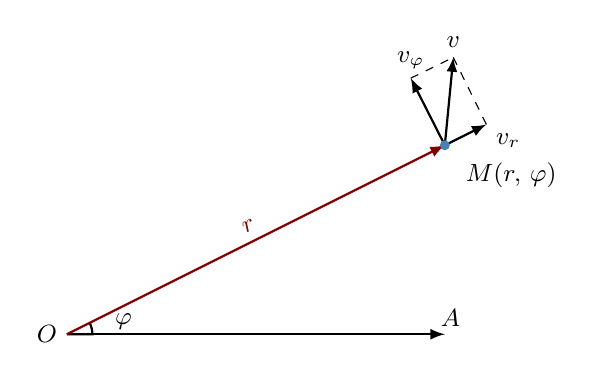
\begin{tikzpicture}[scale=1.2,font=\small]

\draw [shift={(0.,0.)},thick] (0,0) -- (0.:0.27) arc (0.:26.8:0.27);
\draw [thick,-latex] (0.,0.)-- (4.,0.);
\draw [thick,Maroon,-latex] (0.,0.)-- (4.,2.)node [midway, above, sloped] (TextNode){$\vb{r}$} ;
\draw [thick,-latex] (4.,2.)-- (4.44,2.22);
\draw [thick,latex-] (3.64,2.71)-- (4.,2.);
\draw [thick,-latex] (4.,2.)-- (4.09,2.93);
\draw [dashed] (3.64,2.71)-- (4.09,2.93);
\draw [dashed] (4.09,2.93)-- (4.44,2.22);
%\begin{scriptsize}
%\draw [fill=xdxdff] (0.,0.) circle (2.5pt);
\draw[left] (0,0) node {$O$};
%\draw [fill=xdxdff] (4.,0.) circle (2.5pt);
\draw[] (4.06,0.17) node {$A$};
\fill [SteelBlue] (4,2) circle (1.5pt);
\draw[below right] (4.12,1.92) node {$M(r,\,\varphi)$};
\draw[below right] (4.44,2.22) node {$\vb{v}_{r}$};
\draw[above] (3.64,2.71) node {$\vb{v}_{\varphi}$};
\draw[above] (4.09,2.93) node {$\vb{v}$};
\draw[] (0.60,0.13) node {$\varphi$};
%\end{scriptsize}
\end{tikzpicture}
